\documentclass[paper=a4, fontsize=11pt]{scrartcl}
\usepackage[T1]{fontenc}
\usepackage[utf8]{inputenc}
\usepackage{lmodern}
\usepackage{multirow}
\usepackage[table,xcdraw]{xcolor}
\usepackage[spanish]{babel}
\usepackage{cite}
\usepackage{amsmath,amsfonts,amsthm} % Math packages
\usepackage{graphics,graphicx, float} %para incluir imágenes y colocarlas
\usepackage[backref,colorlinks=true,linkcolor=black,urlcolor=blue,citecolor=blue]{hyperref} %Para crear enlaces en el pdf
\usepackage[noabbrev,spanish]{cleveref}
\usepackage{url}
\usepackage[shortlabels]{enumitem}
\usepackage{appendix}
\usepackage{eurosym}
\usepackage{epsfig}
\usepackage{caption}
\usepackage{subcaption}

\renewcommand{\appendixname}{Anexo}
\renewcommand{\appendixtocname}{Anexo}
\renewcommand{\appendixpagename}{Anexo}

\numberwithin{figure}{section} % Number figures within sections (i.e. 1.1, 1.2, 2.1, 2.2 instead of 1, 2, 3, 4)
\numberwithin{table}{section} % Number tables within sections (i.e. 1.1, 1.2, 2.1, 2.2 instead of 1, 2, 3, 4)
\newcommand{\horrule}[1]{\rule{\linewidth}{#1}} % Create horizontal rule command with 1 argument of height

\title{
    \normalfont \normalsize
    \textsc{{\bf Ingeniería de Servidores (2015-2016)} \\ Grado en Ingeniería Informática \\ Universidad de Granada} \\ [25pt] % Your university, school and/or department name(s)
    \horrule{0.5pt} \\[0.4cm] % Thin top horizontal rule
    \huge Memoria Práctica 5 \\ % The assignment title
    \horrule{2pt} \\[0.5cm] % Thick bottom horizontal rule
}
\author{Antonio de la Vega Jiménez }

%*************************************************************


\begin{document}

\maketitle % Muestra el Título
\newpage %inserta un salto de página
\tableofcontents % para generar el índice de contenidos
\listoffigures
\newpage
%*************************************************************

\section{Parámetros del sistema y su edición}
\subsection{Sistemas UNIX: Sysctl y /proc}
\subsubsection{Cuestión 1}
\textit{Al modificar los valores del kernel de este modo, no logramos que persistan después de reiniciar la máquina. ¿Qué archivo hay que editar para que los cambios sean permanentes?}
\newline

Para que los cambios realizados en los parámetros del kernel sen permanentes, es necesario realizarlos en el archivo /etc/sysctl.conf \cite{s1} \cite{s2}

\subsubsection{Cuestión 2}
\textit{¿Con qué opción se muestran todos los parámetros modificables en tiempo de ejecución? Elija dos parámetros y expliqué, en dos líneas, qué función tienen.}
\newline

El comando para que se muestren todos los parámetros modificables es \texttt{sysctl -a} \cite{s3}. Uno de los parámetros más interesantes que he encontrado es vm.\texttt{swappiness}, este parámetro indica al kernel como administrar la RAM, puede tomar un valor entre 0 y 100,  si se usa un valor pequeño el kernel intentará no hacer uso de swap mientras que si se usa un valor grande hará más uso de swap.\cite{sw} Otro parámetro es net.ipv4.\texttt{icmp\_echo\_ignore\_broadcasts} que si tiene un valor distinto de 0 hará que el kernel ignore todas las peticiones de ICMP ECHO y TIMESTAMP enviadas por multicast o broadcast.\cite{net}

\subsection{Windows: Edición del registro}
\subsubsection{Cuestión 3}
\textit{Realice una copia de seguridad del registro y restaurela, ilustre el proceso con capturas.}

El proceso para realizar una copia de seguridad descrito en consiste en exportar el registro. \cite{bac} El proceso seguido para llevar a cabo esto se muestra y describe en las \crefrange{fig1}{fig3}.
\begin{figure}[H]
  \begin{center}
    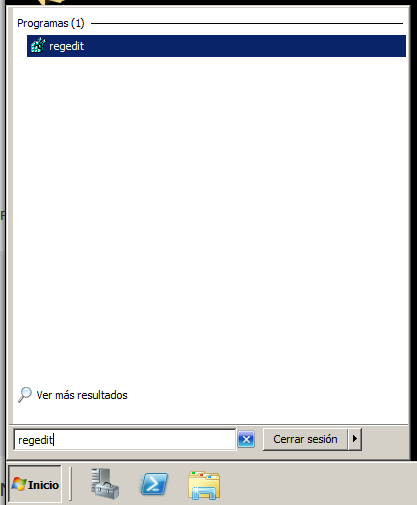
\includegraphics[width=0.5\textwidth]{imagenes/1}
    \caption{Primer paso: abrir el editor del registro de Windows.}
    \label{fig1}
  \end{center}
\end{figure}

\begin{figure}[H]
  \begin{center}
    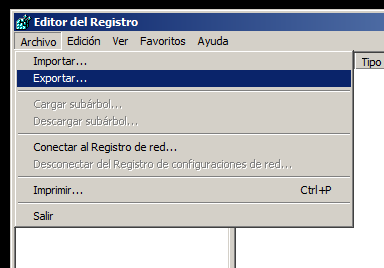
\includegraphics[width=0.5\textwidth]{imagenes/2}
    \caption{Segundo paso: exportar el registro.}
    \label{fig2}
  \end{center}
\end{figure}

\begin{figure}[H]
  \begin{center}
    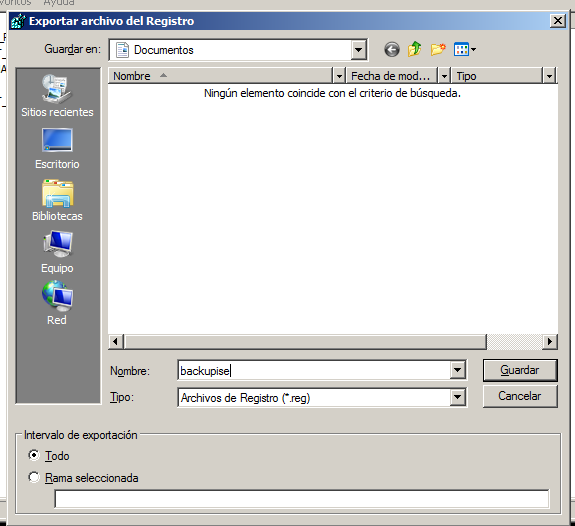
\includegraphics[width=0.5\textwidth]{imagenes/3}
    \caption{Tercer paso: indicar donde queremos guardar la copia del registro.}
    \label{fig3}
  \end{center}
\end{figure}

Una vez que hemos exportado el registro ya tenemos una copia de seguridad, ahora para probar que funciona vamos a modificar un valor del registro y luego vamos a restaurar el registro guardado para ver si el valor vuelve a su estado original. En las \crefrange{fig4}{fig5} se muestra como se modifica el registro.

\begin{figure}[H]
  \begin{center}
    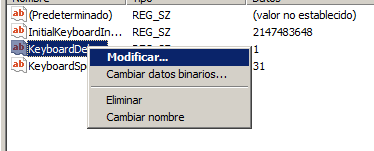
\includegraphics[width=0.5\textwidth]{imagenes/4}
    \caption{Modificación de un valor del registro.}
    \label{fig4}
  \end{center}
\end{figure}

\begin{figure}[H]
  \begin{center}
    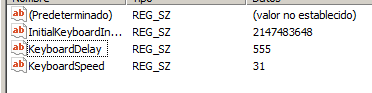
\includegraphics[width=0.5\textwidth]{imagenes/5}
    \caption{Resultado de la modificación.}
    \label{fig5}
  \end{center}
\end{figure}

Ahora que ya hemos modificado el registro, procedemos a restaurar el registro anterior y a comprobar si se ha realizado correctamente la recuperacion como se muestra en las \crefrange{fig6}{fig7}.
\begin{figure}[H]
  \begin{center}
    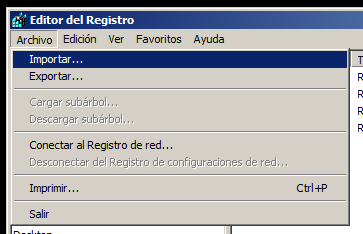
\includegraphics[width=0.5\textwidth]{imagenes/6}
    \caption{Para restaurar el registro pinchamos en importar e importamos el archivo guardado en \ref{fig3}.}
    \label{fig6}
  \end{center}
\end{figure}

\begin{figure}[H]
  \begin{center}
    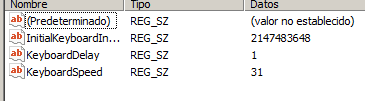
\includegraphics[width=0.5\textwidth]{imagenes/7}
    \caption{Comprobamos que se ha restaurado el valor de Keyboard Delay a su estado original (1).}
    \label{fig7}
  \end{center}
\end{figure}



\subsubsection{Cuestión 4}
\textit{¿Cómo se abre una consola en Windows? ¿Qué comando hay que ejecutar para editar el registro? Muestre su ejecución con capturas de pantalla.}
\newline

Para abrir una consola en Windows debemos dirigirnos a inicio y buscar cmd o Símbolo del sistema y ejecutar la aplicación, también existe la posibilidad de abrir la consola PowerShell si esta disponible.\cite{cmd} Para editar el registro debemos ejecutar el comando \texttt{REG} \cite{reg1}\cite{reg2} mostrado en la \cref{fig8}.

\begin{figure}[H]
  \begin{center}
    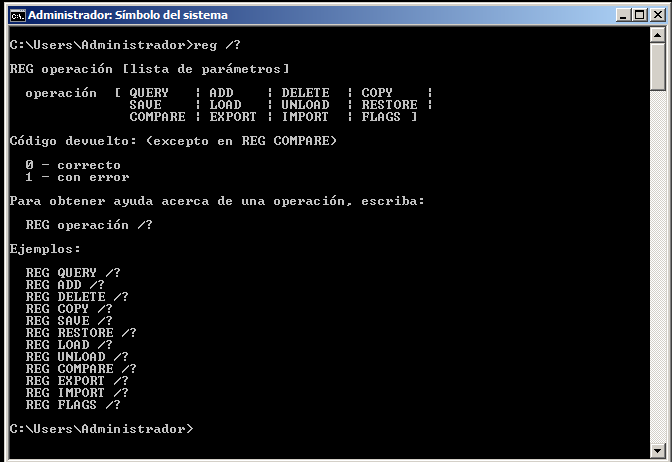
\includegraphics[width=0.5\textwidth]{imagenes/8}
    \caption{Comando REG.}
    \label{fig8}
  \end{center}
\end{figure}

\subsubsection{Cuestión 5}
\textit{Las cadenas de caracteres y valores numéricos tienen distintos tipos. Busque en la documentación de Microsoft y liste todos los tipos de valores.}

Los tipos exixstentes son: \cite{reg3}
\begin{enumerate}
    \item \textbf{REG\_BINARY: }Dato binario de cualquier forma.
    \item \textbf{REG\_DWORD: }Número de 32 bits.
    \item \textbf{REG\_DWORD\_LITTLE\_ENDIAN: }Número de 32 bits en formato little-endian.
    \item \textbf{REG\_DWORD\_BIG\_ENDIAN:} Número de 32 bits en formato big-endian.
    \item \textbf{REG\_EXPAND\_SZ: }Cadena terminada en null que contiene referencias sin expandir a variables de entorno.
    \item \textbf{REG\_LINK: }Cadena terminada en null que contiene la ruta de un enlace simbólico.
    \item \textbf{REG\_MULTI\_SZ:} Secuencia de cadenas terminadas en null terminada por una cadena vacía (\\0).
    \item \textbf{REG\_NONE: }Sin tipo de valor definido.
    \item \textbf{REG\_QWORD: }Numero de 64 bits.
    \item \textbf{REG\_QWORD\_LITTLE\_ENDIAN:} Numero de 64 bits en formato little-endian.
    \item \textbf{REG\_SZ: }Cadena terminada en null.
\end{enumerate}


\section{Mejora de un servivio concreto}
\subsection{Servidor web: Apache e IIS}
\subsubsection{Cuestión 6}
\textit{Enumere qué elementos se pueden configurar en Apache y en IIS para que Moodle funcione mejor.}

En Apache se pueden modificar numerosos parámetros para que funcione mejor, como son: \cite{moda}
\begin{itemize}
    \item \textbf{MaxClient }que debe ser ajustado según la formula $MaxCliente = Memoria\ total\ disponible * 80 \% / Memoria\ máxima\ usada\ por\ el\ proceso\ apache$
    \item Reducir el número de \textbf{modulos que Apache }carga.
    \item Bajar el valor de \textbf{MaxRequestPerChild} a 20-30.
    \item Establecer \textbf{KeepAlive} a off.
    \item Bajar \textbf{KeepAliveTimeout} a 2-5 segundos.
    \item Establecer \textbf{AllowOverrride} a none.
    \item Establecer \textbf{ExtendedStatus} y \textbf{HostnameLookups} a off.
    \item \textbf{Comprimir} las respuestas para bajar el tiempo de respuesta.
\end{itemize}

Por otro lado para IIS se pueden realizar modificaciones como: \cite{modi}
\begin{itemize}
    \item Establecer \textbf{ListenBackLog} a un valor entre 2 y 5.
    \item Ajustar el valor de \textbf{MenCacheSize}.
    \item Cambiar \textbf{MaxCachedFileSize }para ajustar el tamaño máximo de un archivo en caché.
    \item Crear una nueva DWORD llamada \textbf{ObjectCacheTTL} para modificar el tiempo que los objetos estran en caché.
\end{itemize}

\subsubsection{Cuestión 7}
\textit{Ajuste la compresión en el servidor y analice su
comportamiento usando varios valores para el tamaño a de archivo partir del cual comprimir. Para comprobar que está comprimiendo puede usar el navegador o comandos como curl (see url) o lynx. Muestre capturas de pantalla de todo el proceso.}

En esta cuestión voy a modificar la compresión en IIS, para ello nos dirigimos a administrador de IIS y pinchamos en compresión ( \cref{fig9}), una vez ahí seleccionamos el tamaño en bytes a partir del cual se va a comprimir y aplicamos los cambios ( \cref{fig10}). Con el parámetro modificado para que comprima los archivos con un tamaño superior a un byte nos dirigimos al navegador y verificamos que la web servida por IIS ha sido comprimida como se ve en la \\cref{fig11}.

\subsection{Servicios de libre elección}
\subsubsection{Cuestión 8}
\textit{Usted parte de un SO con ciertos parámetros definidos en la instalación (Práctica 1), ya sabe instalar servicios (Práctica 2) y cómo monitorizarlos (Práctica 3) cuando los somete a cargas (Práctica 4). Al igual que ha visto cómo se puede mejorar un servidor web (Práctica 5 Sección 3.1), elija un servicio (el que usted quiera) y modifique un parámetro para mejorar su comportamiento. (9.b) Monitorice el servicio antes y después de la modificación del parámetro aplicando cargas al sistema (antes y después) mostrando los resultados de la monitorización.}
\subsubsection{Cuestión opcional 1}
\textit{Realice lo mismo que en la cuestión 8 pero para otro servicio.}
%*************************************************************
\newpage
\bibliographystyle{ieeetr}
\bibliography{citas}

\end{document}
